\documentclass[11pt]{article}
\usepackage{sectsty}
\allsectionsfont{\color{blue}\fontfamily{lmss}\selectfont}
\usepackage{fontspec}
\setmainfont{XCharter}

\usepackage{listings}
\lstset{
basicstyle=\small\ttfamily,
tabsize=8,
columns=flexible,
breaklines=true,
frame=tb,
rulecolor=\color[rgb]{0.8,0.8,0.7},
backgroundcolor=\color[rgb]{1,1,0.91},
postbreak=\raisebox{0ex}[0ex][0ex]{\ensuremath{\color{red}\hookrightarrow\space}}
}
\usepackage{fontawesome}


\usepackage{mdframed}
\newmdenv[
  backgroundcolor=gray,
  fontcolor=white,
  nobreak=true,
]{terminalinput}



\usepackage{parskip}


    \usepackage[breakable]{tcolorbox}
    \usepackage{parskip} % Stop auto-indenting (to mimic markdown behaviour)

    \usepackage{iftex}
    \ifPDFTeX
    	\usepackage[T1]{fontenc}
    	\usepackage{mathpazo}
    \else
    	\usepackage{fontspec}
    \fi

    % Basic figure setup, for now with no caption control since it's done
    % automatically by Pandoc (which extracts ![](path) syntax from Markdown).
    \usepackage{graphicx}
    % Maintain compatibility with old templates. Remove in nbconvert 6.0
    \let\Oldincludegraphics\includegraphics
    % Ensure that by default, figures have no caption (until we provide a
    % proper Figure object with a Caption API and a way to capture that
    % in the conversion process - todo).
    \usepackage{caption}
    \DeclareCaptionFormat{nocaption}{}
    \captionsetup{format=nocaption,aboveskip=0pt,belowskip=0pt}

    \usepackage{float}
    \floatplacement{figure}{H} % forces figures to be placed at the correct location
    \usepackage{xcolor} % Allow colors to be defined
    \usepackage{enumerate} % Needed for markdown enumerations to work
    \usepackage{geometry} % Used to adjust the document margins
    \usepackage{amsmath} % Equations
    \usepackage{amssymb} % Equations
    \usepackage{textcomp} % defines textquotesingle
    % Hack from http://tex.stackexchange.com/a/47451/13684:
    \AtBeginDocument{%
        \def\PYZsq{\textquotesingle}% Upright quotes in Pygmentized code
    }
    \usepackage{upquote} % Upright quotes for verbatim code
    \usepackage{eurosym} % defines \euro
    \usepackage[mathletters]{ucs} % Extended unicode (utf-8) support
    \usepackage{fancyvrb} % verbatim replacement that allows latex
    \usepackage{grffile} % extends the file name processing of package graphics
                         % to support a larger range
    \makeatletter % fix for old versions of grffile with XeLaTeX
    \@ifpackagelater{grffile}{2019/11/01}
    {
      % Do nothing on new versions
    }
    {
      \def\Gread@@xetex#1{%
        \IfFileExists{"\Gin@base".bb}%
        {\Gread@eps{\Gin@base.bb}}%
        {\Gread@@xetex@aux#1}%
      }
    }
    \makeatother
    \usepackage[Export]{adjustbox} % Used to constrain images to a maximum size
    \adjustboxset{max size={0.9\linewidth}{0.9\paperheight}}

    % The hyperref package gives us a pdf with properly built
    % internal navigation ('pdf bookmarks' for the table of contents,
    % internal cross-reference links, web links for URLs, etc.)
    \usepackage{hyperref}
    % The default LaTeX title has an obnoxious amount of whitespace. By default,
    % titling removes some of it. It also provides customization options.
    \usepackage{titling}
    \usepackage{longtable} % longtable support required by pandoc >1.10
    \usepackage{booktabs}  % table support for pandoc > 1.12.2
    \usepackage[inline]{enumitem} % IRkernel/repr support (it uses the enumerate* environment)
    \usepackage[normalem]{ulem} % ulem is needed to support strikethroughs (\sout)
                                % normalem makes italics be italics, not underlines
    \usepackage{mathrsfs}



    % Colors for the hyperref package
    \definecolor{urlcolor}{rgb}{0,.145,.698}
    \definecolor{linkcolor}{rgb}{.71,0.21,0.01}
    \definecolor{citecolor}{rgb}{.12,.54,.11}

    % ANSI colors
    \definecolor{ansi-black}{HTML}{3E424D}
    \definecolor{ansi-black-intense}{HTML}{282C36}
    \definecolor{ansi-red}{HTML}{E75C58}
    \definecolor{ansi-red-intense}{HTML}{B22B31}
    \definecolor{ansi-green}{HTML}{00A250}
    \definecolor{ansi-green-intense}{HTML}{007427}
    \definecolor{ansi-yellow}{HTML}{DDB62B}
    \definecolor{ansi-yellow-intense}{HTML}{B27D12}
    \definecolor{ansi-blue}{HTML}{208FFB}
    \definecolor{ansi-blue-intense}{HTML}{0065CA}
    \definecolor{ansi-magenta}{HTML}{D160C4}
    \definecolor{ansi-magenta-intense}{HTML}{A03196}
    \definecolor{ansi-cyan}{HTML}{60C6C8}
    \definecolor{ansi-cyan-intense}{HTML}{258F8F}
    \definecolor{ansi-white}{HTML}{C5C1B4}
    \definecolor{ansi-white-intense}{HTML}{A1A6B2}
    \definecolor{ansi-default-inverse-fg}{HTML}{FFFFFF}
    \definecolor{ansi-default-inverse-bg}{HTML}{000000}

    % common color for the border for error outputs.
    \definecolor{outerrorbackground}{HTML}{FFDFDF}

    % commands and environments needed by pandoc snippets
    % extracted from the output of `pandoc -s`
    \providecommand{\tightlist}{%
      \setlength{\itemsep}{0pt}\setlength{\parskip}{0pt}}
    \DefineVerbatimEnvironment{Highlighting}{Verbatim}{commandchars=\\\{\}}
    % Add ',fontsize=\small' for more characters per line
    \newenvironment{Shaded}{}{}
    \newcommand{\KeywordTok}[1]{\textcolor[rgb]{0.00,0.44,0.13}{\textbf{{#1}}}}
    \newcommand{\DataTypeTok}[1]{\textcolor[rgb]{0.56,0.13,0.00}{{#1}}}
    \newcommand{\DecValTok}[1]{\textcolor[rgb]{0.25,0.63,0.44}{{#1}}}
    \newcommand{\BaseNTok}[1]{\textcolor[rgb]{0.25,0.63,0.44}{{#1}}}
    \newcommand{\FloatTok}[1]{\textcolor[rgb]{0.25,0.63,0.44}{{#1}}}
    \newcommand{\CharTok}[1]{\textcolor[rgb]{0.25,0.44,0.63}{{#1}}}
    \newcommand{\StringTok}[1]{\textcolor[rgb]{0.25,0.44,0.63}{{#1}}}
    \newcommand{\CommentTok}[1]{\textcolor[rgb]{0.38,0.63,0.69}{\textit{{#1}}}}
    \newcommand{\OtherTok}[1]{\textcolor[rgb]{0.00,0.44,0.13}{{#1}}}
    \newcommand{\AlertTok}[1]{\textcolor[rgb]{1.00,0.00,0.00}{\textbf{{#1}}}}
    \newcommand{\FunctionTok}[1]{\textcolor[rgb]{0.02,0.16,0.49}{{#1}}}
    \newcommand{\RegionMarkerTok}[1]{{#1}}
    \newcommand{\ErrorTok}[1]{\textcolor[rgb]{1.00,0.00,0.00}{\textbf{{#1}}}}
    \newcommand{\NormalTok}[1]{{#1}}

    % Additional commands for more recent versions of Pandoc
    \newcommand{\ConstantTok}[1]{\textcolor[rgb]{0.53,0.00,0.00}{{#1}}}
    \newcommand{\SpecialCharTok}[1]{\textcolor[rgb]{0.25,0.44,0.63}{{#1}}}
    \newcommand{\VerbatimStringTok}[1]{\textcolor[rgb]{0.25,0.44,0.63}{{#1}}}
    \newcommand{\SpecialStringTok}[1]{\textcolor[rgb]{0.73,0.40,0.53}{{#1}}}
    \newcommand{\ImportTok}[1]{{#1}}
    \newcommand{\DocumentationTok}[1]{\textcolor[rgb]{0.73,0.13,0.13}{\textit{{#1}}}}
    \newcommand{\AnnotationTok}[1]{\textcolor[rgb]{0.38,0.63,0.69}{\textbf{\textit{{#1}}}}}
    \newcommand{\CommentVarTok}[1]{\textcolor[rgb]{0.38,0.63,0.69}{\textbf{\textit{{#1}}}}}
    \newcommand{\VariableTok}[1]{\textcolor[rgb]{0.10,0.09,0.49}{{#1}}}
    \newcommand{\ControlFlowTok}[1]{\textcolor[rgb]{0.00,0.44,0.13}{\textbf{{#1}}}}
    \newcommand{\OperatorTok}[1]{\textcolor[rgb]{0.40,0.40,0.40}{{#1}}}
    \newcommand{\BuiltInTok}[1]{{#1}}
    \newcommand{\ExtensionTok}[1]{{#1}}
    \newcommand{\PreprocessorTok}[1]{\textcolor[rgb]{0.74,0.48,0.00}{{#1}}}
    \newcommand{\AttributeTok}[1]{\textcolor[rgb]{0.49,0.56,0.16}{{#1}}}
    \newcommand{\InformationTok}[1]{\textcolor[rgb]{0.38,0.63,0.69}{\textbf{\textit{{#1}}}}}
    \newcommand{\WarningTok}[1]{\textcolor[rgb]{0.38,0.63,0.69}{\textbf{\textit{{#1}}}}}


    % Define a nice break command that doesn't care if a line doesn't already
    % exist.
    \def\br{\hspace*{\fill} \\* }
    % Math Jax compatibility definitions
    \def\gt{>}
    \def\lt{<}
    \let\Oldtex\TeX
    \let\Oldlatex\LaTeX
    \renewcommand{\TeX}{\textrm{\Oldtex}}
    \renewcommand{\LaTeX}{\textrm{\Oldlatex}}
    % Document parameters
    % Document title
    \title{answers}





% Pygments definitions
\makeatletter
\def\PY@reset{\let\PY@it=\relax \let\PY@bf=\relax%
    \let\PY@ul=\relax \let\PY@tc=\relax%
    \let\PY@bc=\relax \let\PY@ff=\relax}
\def\PY@tok#1{\csname PY@tok@#1\endcsname}
\def\PY@toks#1+{\ifx\relax#1\empty\else%
    \PY@tok{#1}\expandafter\PY@toks\fi}
\def\PY@do#1{\PY@bc{\PY@tc{\PY@ul{%
    \PY@it{\PY@bf{\PY@ff{#1}}}}}}}
\def\PY#1#2{\PY@reset\PY@toks#1+\relax+\PY@do{#2}}

\expandafter\def\csname PY@tok@w\endcsname{\def\PY@tc##1{\textcolor[rgb]{0.73,0.73,0.73}{##1}}}
\expandafter\def\csname PY@tok@c\endcsname{\let\PY@it=\textit\def\PY@tc##1{\textcolor[rgb]{0.25,0.50,0.50}{##1}}}
\expandafter\def\csname PY@tok@cp\endcsname{\def\PY@tc##1{\textcolor[rgb]{0.74,0.48,0.00}{##1}}}
\expandafter\def\csname PY@tok@k\endcsname{\let\PY@bf=\textbf\def\PY@tc##1{\textcolor[rgb]{0.00,0.50,0.00}{##1}}}
\expandafter\def\csname PY@tok@kp\endcsname{\def\PY@tc##1{\textcolor[rgb]{0.00,0.50,0.00}{##1}}}
\expandafter\def\csname PY@tok@kt\endcsname{\def\PY@tc##1{\textcolor[rgb]{0.69,0.00,0.25}{##1}}}
\expandafter\def\csname PY@tok@o\endcsname{\def\PY@tc##1{\textcolor[rgb]{0.40,0.40,0.40}{##1}}}
\expandafter\def\csname PY@tok@ow\endcsname{\let\PY@bf=\textbf\def\PY@tc##1{\textcolor[rgb]{0.67,0.13,1.00}{##1}}}
\expandafter\def\csname PY@tok@nb\endcsname{\def\PY@tc##1{\textcolor[rgb]{0.00,0.50,0.00}{##1}}}
\expandafter\def\csname PY@tok@nf\endcsname{\def\PY@tc##1{\textcolor[rgb]{0.00,0.00,1.00}{##1}}}
\expandafter\def\csname PY@tok@nc\endcsname{\let\PY@bf=\textbf\def\PY@tc##1{\textcolor[rgb]{0.00,0.00,1.00}{##1}}}
\expandafter\def\csname PY@tok@nn\endcsname{\let\PY@bf=\textbf\def\PY@tc##1{\textcolor[rgb]{0.00,0.00,1.00}{##1}}}
\expandafter\def\csname PY@tok@ne\endcsname{\let\PY@bf=\textbf\def\PY@tc##1{\textcolor[rgb]{0.82,0.25,0.23}{##1}}}
\expandafter\def\csname PY@tok@nv\endcsname{\def\PY@tc##1{\textcolor[rgb]{0.10,0.09,0.49}{##1}}}
\expandafter\def\csname PY@tok@no\endcsname{\def\PY@tc##1{\textcolor[rgb]{0.53,0.00,0.00}{##1}}}
\expandafter\def\csname PY@tok@nl\endcsname{\def\PY@tc##1{\textcolor[rgb]{0.63,0.63,0.00}{##1}}}
\expandafter\def\csname PY@tok@ni\endcsname{\let\PY@bf=\textbf\def\PY@tc##1{\textcolor[rgb]{0.60,0.60,0.60}{##1}}}
\expandafter\def\csname PY@tok@na\endcsname{\def\PY@tc##1{\textcolor[rgb]{0.49,0.56,0.16}{##1}}}
\expandafter\def\csname PY@tok@nt\endcsname{\let\PY@bf=\textbf\def\PY@tc##1{\textcolor[rgb]{0.00,0.50,0.00}{##1}}}
\expandafter\def\csname PY@tok@nd\endcsname{\def\PY@tc##1{\textcolor[rgb]{0.67,0.13,1.00}{##1}}}
\expandafter\def\csname PY@tok@s\endcsname{\def\PY@tc##1{\textcolor[rgb]{0.73,0.13,0.13}{##1}}}
\expandafter\def\csname PY@tok@sd\endcsname{\let\PY@it=\textit\def\PY@tc##1{\textcolor[rgb]{0.73,0.13,0.13}{##1}}}
\expandafter\def\csname PY@tok@si\endcsname{\let\PY@bf=\textbf\def\PY@tc##1{\textcolor[rgb]{0.73,0.40,0.53}{##1}}}
\expandafter\def\csname PY@tok@se\endcsname{\let\PY@bf=\textbf\def\PY@tc##1{\textcolor[rgb]{0.73,0.40,0.13}{##1}}}
\expandafter\def\csname PY@tok@sr\endcsname{\def\PY@tc##1{\textcolor[rgb]{0.73,0.40,0.53}{##1}}}
\expandafter\def\csname PY@tok@ss\endcsname{\def\PY@tc##1{\textcolor[rgb]{0.10,0.09,0.49}{##1}}}
\expandafter\def\csname PY@tok@sx\endcsname{\def\PY@tc##1{\textcolor[rgb]{0.00,0.50,0.00}{##1}}}
\expandafter\def\csname PY@tok@m\endcsname{\def\PY@tc##1{\textcolor[rgb]{0.40,0.40,0.40}{##1}}}
\expandafter\def\csname PY@tok@gh\endcsname{\let\PY@bf=\textbf\def\PY@tc##1{\textcolor[rgb]{0.00,0.00,0.50}{##1}}}
\expandafter\def\csname PY@tok@gu\endcsname{\let\PY@bf=\textbf\def\PY@tc##1{\textcolor[rgb]{0.50,0.00,0.50}{##1}}}
\expandafter\def\csname PY@tok@gd\endcsname{\def\PY@tc##1{\textcolor[rgb]{0.63,0.00,0.00}{##1}}}
\expandafter\def\csname PY@tok@gi\endcsname{\def\PY@tc##1{\textcolor[rgb]{0.00,0.63,0.00}{##1}}}
\expandafter\def\csname PY@tok@gr\endcsname{\def\PY@tc##1{\textcolor[rgb]{1.00,0.00,0.00}{##1}}}
\expandafter\def\csname PY@tok@ge\endcsname{\let\PY@it=\textit}
\expandafter\def\csname PY@tok@gs\endcsname{\let\PY@bf=\textbf}
\expandafter\def\csname PY@tok@gp\endcsname{\let\PY@bf=\textbf\def\PY@tc##1{\textcolor[rgb]{0.00,0.00,0.50}{##1}}}
\expandafter\def\csname PY@tok@go\endcsname{\def\PY@tc##1{\textcolor[rgb]{0.53,0.53,0.53}{##1}}}
\expandafter\def\csname PY@tok@gt\endcsname{\def\PY@tc##1{\textcolor[rgb]{0.00,0.27,0.87}{##1}}}
\expandafter\def\csname PY@tok@err\endcsname{\def\PY@bc##1{\setlength{\fboxsep}{0pt}\fcolorbox[rgb]{1.00,0.00,0.00}{1,1,1}{\strut ##1}}}
\expandafter\def\csname PY@tok@kc\endcsname{\let\PY@bf=\textbf\def\PY@tc##1{\textcolor[rgb]{0.00,0.50,0.00}{##1}}}
\expandafter\def\csname PY@tok@kd\endcsname{\let\PY@bf=\textbf\def\PY@tc##1{\textcolor[rgb]{0.00,0.50,0.00}{##1}}}
\expandafter\def\csname PY@tok@kn\endcsname{\let\PY@bf=\textbf\def\PY@tc##1{\textcolor[rgb]{0.00,0.50,0.00}{##1}}}
\expandafter\def\csname PY@tok@kr\endcsname{\let\PY@bf=\textbf\def\PY@tc##1{\textcolor[rgb]{0.00,0.50,0.00}{##1}}}
\expandafter\def\csname PY@tok@bp\endcsname{\def\PY@tc##1{\textcolor[rgb]{0.00,0.50,0.00}{##1}}}
\expandafter\def\csname PY@tok@fm\endcsname{\def\PY@tc##1{\textcolor[rgb]{0.00,0.00,1.00}{##1}}}
\expandafter\def\csname PY@tok@vc\endcsname{\def\PY@tc##1{\textcolor[rgb]{0.10,0.09,0.49}{##1}}}
\expandafter\def\csname PY@tok@vg\endcsname{\def\PY@tc##1{\textcolor[rgb]{0.10,0.09,0.49}{##1}}}
\expandafter\def\csname PY@tok@vi\endcsname{\def\PY@tc##1{\textcolor[rgb]{0.10,0.09,0.49}{##1}}}
\expandafter\def\csname PY@tok@vm\endcsname{\def\PY@tc##1{\textcolor[rgb]{0.10,0.09,0.49}{##1}}}
\expandafter\def\csname PY@tok@sa\endcsname{\def\PY@tc##1{\textcolor[rgb]{0.73,0.13,0.13}{##1}}}
\expandafter\def\csname PY@tok@sb\endcsname{\def\PY@tc##1{\textcolor[rgb]{0.73,0.13,0.13}{##1}}}
\expandafter\def\csname PY@tok@sc\endcsname{\def\PY@tc##1{\textcolor[rgb]{0.73,0.13,0.13}{##1}}}
\expandafter\def\csname PY@tok@dl\endcsname{\def\PY@tc##1{\textcolor[rgb]{0.73,0.13,0.13}{##1}}}
\expandafter\def\csname PY@tok@s2\endcsname{\def\PY@tc##1{\textcolor[rgb]{0.73,0.13,0.13}{##1}}}
\expandafter\def\csname PY@tok@sh\endcsname{\def\PY@tc##1{\textcolor[rgb]{0.73,0.13,0.13}{##1}}}
\expandafter\def\csname PY@tok@s1\endcsname{\def\PY@tc##1{\textcolor[rgb]{0.73,0.13,0.13}{##1}}}
\expandafter\def\csname PY@tok@mb\endcsname{\def\PY@tc##1{\textcolor[rgb]{0.40,0.40,0.40}{##1}}}
\expandafter\def\csname PY@tok@mf\endcsname{\def\PY@tc##1{\textcolor[rgb]{0.40,0.40,0.40}{##1}}}
\expandafter\def\csname PY@tok@mh\endcsname{\def\PY@tc##1{\textcolor[rgb]{0.40,0.40,0.40}{##1}}}
\expandafter\def\csname PY@tok@mi\endcsname{\def\PY@tc##1{\textcolor[rgb]{0.40,0.40,0.40}{##1}}}
\expandafter\def\csname PY@tok@il\endcsname{\def\PY@tc##1{\textcolor[rgb]{0.40,0.40,0.40}{##1}}}
\expandafter\def\csname PY@tok@mo\endcsname{\def\PY@tc##1{\textcolor[rgb]{0.40,0.40,0.40}{##1}}}
\expandafter\def\csname PY@tok@ch\endcsname{\let\PY@it=\textit\def\PY@tc##1{\textcolor[rgb]{0.25,0.50,0.50}{##1}}}
\expandafter\def\csname PY@tok@cm\endcsname{\let\PY@it=\textit\def\PY@tc##1{\textcolor[rgb]{0.25,0.50,0.50}{##1}}}
\expandafter\def\csname PY@tok@cpf\endcsname{\let\PY@it=\textit\def\PY@tc##1{\textcolor[rgb]{0.25,0.50,0.50}{##1}}}
\expandafter\def\csname PY@tok@c1\endcsname{\let\PY@it=\textit\def\PY@tc##1{\textcolor[rgb]{0.25,0.50,0.50}{##1}}}
\expandafter\def\csname PY@tok@cs\endcsname{\let\PY@it=\textit\def\PY@tc##1{\textcolor[rgb]{0.25,0.50,0.50}{##1}}}

\def\PYZbs{\char`\\}
\def\PYZus{\char`\_}
\def\PYZob{\char`\{}
\def\PYZcb{\char`\}}
\def\PYZca{\char`\^}
\def\PYZam{\char`\&}
\def\PYZlt{\char`\<}
\def\PYZgt{\char`\>}
\def\PYZsh{\char`\#}
\def\PYZpc{\char`\%}
\def\PYZdl{\char`\$}
\def\PYZhy{\char`\-}
\def\PYZsq{\char`\'}
\def\PYZdq{\char`\"}
\def\PYZti{\char`\~}
% for compatibility with earlier versions
\def\PYZat{@}
\def\PYZlb{[}
\def\PYZrb{]}
\makeatother


    % For linebreaks inside Verbatim environment from package fancyvrb.
    \makeatletter
        \newbox\Wrappedcontinuationbox
        \newbox\Wrappedvisiblespacebox
        \newcommand*\Wrappedvisiblespace {\textcolor{red}{\textvisiblespace}}
        \newcommand*\Wrappedcontinuationsymbol {\textcolor{red}{\llap{\tiny$\m@th\hookrightarrow$}}}
        \newcommand*\Wrappedcontinuationindent {3ex }
        \newcommand*\Wrappedafterbreak {\kern\Wrappedcontinuationindent\copy\Wrappedcontinuationbox}
        % Take advantage of the already applied Pygments mark-up to insert
        % potential linebreaks for TeX processing.
        %        {, <, #, %, $, ' and ": go to next line.
        %        _, }, ^, &, >, - and ~: stay at end of broken line.
        % Use of \textquotesingle for straight quote.
        \newcommand*\Wrappedbreaksatspecials {%
            \def\PYGZus{\discretionary{\char`\_}{\Wrappedafterbreak}{\char`\_}}%
            \def\PYGZob{\discretionary{}{\Wrappedafterbreak\char`\{}{\char`\{}}%
            \def\PYGZcb{\discretionary{\char`\}}{\Wrappedafterbreak}{\char`\}}}%
            \def\PYGZca{\discretionary{\char`\^}{\Wrappedafterbreak}{\char`\^}}%
            \def\PYGZam{\discretionary{\char`\&}{\Wrappedafterbreak}{\char`\&}}%
            \def\PYGZlt{\discretionary{}{\Wrappedafterbreak\char`\<}{\char`\<}}%
            \def\PYGZgt{\discretionary{\char`\>}{\Wrappedafterbreak}{\char`\>}}%
            \def\PYGZsh{\discretionary{}{\Wrappedafterbreak\char`\#}{\char`\#}}%
            \def\PYGZpc{\discretionary{}{\Wrappedafterbreak\char`\%}{\char`\%}}%
            \def\PYGZdl{\discretionary{}{\Wrappedafterbreak\char`\$}{\char`\$}}%
            \def\PYGZhy{\discretionary{\char`\-}{\Wrappedafterbreak}{\char`\-}}%
            \def\PYGZsq{\discretionary{}{\Wrappedafterbreak\textquotesingle}{\textquotesingle}}%
            \def\PYGZdq{\discretionary{}{\Wrappedafterbreak\char`\"}{\char`\"}}%
            \def\PYGZti{\discretionary{\char`\~}{\Wrappedafterbreak}{\char`\~}}%
        }
        % Some characters . , ; ? ! / are not pygmentized.
        % This macro makes them "active" and they will insert potential linebreaks
        \newcommand*\Wrappedbreaksatpunct {%
            \lccode`\~`\.\lowercase{\def~}{\discretionary{\hbox{\char`\.}}{\Wrappedafterbreak}{\hbox{\char`\.}}}%
            \lccode`\~`\,\lowercase{\def~}{\discretionary{\hbox{\char`\,}}{\Wrappedafterbreak}{\hbox{\char`\,}}}%
            \lccode`\~`\;\lowercase{\def~}{\discretionary{\hbox{\char`\;}}{\Wrappedafterbreak}{\hbox{\char`\;}}}%
            \lccode`\~`\:\lowercase{\def~}{\discretionary{\hbox{\char`\:}}{\Wrappedafterbreak}{\hbox{\char`\:}}}%
            \lccode`\~`\?\lowercase{\def~}{\discretionary{\hbox{\char`\?}}{\Wrappedafterbreak}{\hbox{\char`\?}}}%
            \lccode`\~`\!\lowercase{\def~}{\discretionary{\hbox{\char`\!}}{\Wrappedafterbreak}{\hbox{\char`\!}}}%
            \lccode`\~`\/\lowercase{\def~}{\discretionary{\hbox{\char`\/}}{\Wrappedafterbreak}{\hbox{\char`\/}}}%
            \catcode`\.\active
            \catcode`\,\active
            \catcode`\;\active
            \catcode`\:\active
            \catcode`\?\active
            \catcode`\!\active
            \catcode`\/\active
            \lccode`\~`\~
        }
    \makeatother

    \let\OriginalVerbatim=\Verbatim
    \makeatletter
    \renewcommand{\Verbatim}[1][1]{%
        %\parskip\z@skip
        \sbox\Wrappedcontinuationbox {\Wrappedcontinuationsymbol}%
        \sbox\Wrappedvisiblespacebox {\FV@SetupFont\Wrappedvisiblespace}%
        \def\FancyVerbFormatLine ##1{\hsize\linewidth
            \vtop{\raggedright\hyphenpenalty\z@\exhyphenpenalty\z@
                \doublehyphendemerits\z@\finalhyphendemerits\z@
                \strut ##1\strut}%
        }%
        % If the linebreak is at a space, the latter will be displayed as visible
        % space at end of first line, and a continuation symbol starts next line.
        % Stretch/shrink are however usually zero for typewriter font.
        \def\FV@Space {%
            \nobreak\hskip\z@ plus\fontdimen3\font minus\fontdimen4\font
            \discretionary{\copy\Wrappedvisiblespacebox}{\Wrappedafterbreak}
            {\kern\fontdimen2\font}%
        }%

        % Allow breaks at special characters using \PYG... macros.
        \Wrappedbreaksatspecials
        % Breaks at punctuation characters . , ; ? ! and / need catcode=\active
        \OriginalVerbatim[#1,codes*=\Wrappedbreaksatpunct]%
    }
    \makeatother

    % Exact colors from NB
    \definecolor{incolor}{HTML}{303F9F}
    \definecolor{outcolor}{HTML}{D84315}
    \definecolor{cellborder}{HTML}{CFCFCF}
    \definecolor{cellbackground}{HTML}{F7F7F7}

    % prompt
    \makeatletter
    \newcommand{\boxspacing}{\kern\kvtcb@left@rule\kern\kvtcb@boxsep}
    \makeatother
    \newcommand{\prompt}[4]{
        {\ttfamily\llap{{\color{#2}[#3]:\hspace{3pt}#4}}\vspace{-\baselineskip}}
    }



    % Prevent overflowing lines due to hard-to-break entities
    \sloppy
    % Setup hyperref package
    \hypersetup{
      breaklinks=true,  % so long urls are correctly broken across lines
      colorlinks=true,
      urlcolor=urlcolor,
      linkcolor=linkcolor,
      citecolor=citecolor,
      }
    % Slightly bigger margins than the latex defaults

    \geometry{verbose,tmargin=1in,bmargin=1in,lmargin=1in,rmargin=1in}



\renewcommand{\PY}[2]{{#2}}
\usepackage{fancyhdr}
\pagestyle{fancy}
\rhead{\color{gray}\sf\small\rightmark}
\lhead{\nouppercase{\color{gray}\sf\small\leftmark}}
\cfoot{\color{gray}\sf\thepage}
\renewcommand{\footrulewidth}{1pt}
\begin{document}





    \hypertarget{answers}{%
\section{Answers}\label{answers}}

To run the commands alongside the answers you must first have run
\textit{all} of the tutorial commands for that section and generated the
output files they reference.

\hypertarget{tutorial-sections}{%
\subsection{Tutorial sections}\label{tutorial-sections}}

\begin{itemize}
\tightlist
\item
  \hyperref[introducing-the-tutorial-dataset]{Introducing the tutorial dataset}
\item
  \hyperref[mapping-rna-seq-reads-to-the-genome-using-hisat2]{Mapping RNA-Seq reads to the genome using HISAT2}
\item
  \hyperref[visualising-transcriptomes-with-igv]{Visualising transcriptomes with IGV}
\item
  \hyperref[transcript-quantification-with-kallisto]{Transcript quantification with Kallisto}
\item
  \hyperref[identifying-differentially-expressed-genes-with-sleuth]{Identifying differentially expressed genes with Sleuth}
\item
  \hyperref[interpreting-the-results]{Interpreting the results}
\item
  \hyperref[normalisation]{Normalisation}
\end{itemize}

    \begin{center}\rule{0.5\linewidth}{0.5pt}\end{center}

Let's go to our \texttt{data} directory.

    \begin{tcolorbox}[breakable, size=fbox, boxrule=1pt, pad at break*=1mm,colback=cellbackground, colframe=cellborder]
\prompt{In}{incolor}{ }{\boxspacing}
\begin{Verbatim}[commandchars=\\\{\}]
\PY{n+nb}{cd} data
\end{Verbatim}
\end{tcolorbox}

    \begin{center}\rule{0.5\linewidth}{0.5pt}\end{center}

    \hypertarget{introducing-the-tutorial-dataset}{%
\subsection{Introducing the tutorial
dataset}\label{introducing-the-tutorial-dataset}}

    \hypertarget{q1-why-is-there-more-than-one-fastq-file-per-sample}{%
\subsubsection{Q1: Why is there more than one FASTQ file per
sample?}\label{q1-why-is-there-more-than-one-fastq-file-per-sample}}

There are \textbf{2} FASTQ files for each sample
e.g.~MT1\_\textbf{1}.fastq and MT1\_\textbf{2}.fastq. This is because
this was \textbf{paired-end} sequence data.

    \begin{tcolorbox}[breakable, size=fbox, boxrule=1pt, pad at break*=1mm,colback=cellbackground, colframe=cellborder]
\prompt{In}{incolor}{ }{\boxspacing}
\begin{Verbatim}[commandchars=\\\{\}]
ls MT1*.fastq
\end{Verbatim}
\end{tcolorbox}

    \begin{tcolorbox}[breakable, size=fbox, boxrule=1pt, pad at break*=1mm,colback=cellbackground, colframe=cellborder]
\prompt{In}{incolor}{ }{\boxspacing}
\begin{Verbatim}[commandchars=\\\{\}]
ls MT1*.fastq \PY{p}{|} wc \PYZhy{}l
\end{Verbatim}
\end{tcolorbox}

    With Illumina paired-end sequencing, you will have a fragment (hopefully
longer than your reads) which is sequenced at both ends. This means that
there will be a ``left'' read (sometimes known as \textit{r1}) and its
corresonding ``right'' read (sometimes known as \textit{r2}). These are
indicated by the \textbf{/1} and \textbf{/2} at the end of the read name
in the **\_1\textbf{.fastq and }\_2**.fastq files respectively.

So, the left read header \_@HS18\_08296:8:1101:1352:48181\#4\_ in
\textbf{MT1\_1.fastq} has the \textbf{/1} suffix:

\begin{verbatim}
@HS18_08296:8:1101:1352:48181#4/1
\end{verbatim}

And, the corresponding right read header in \textbf{MT1\_2.fastq} has
the \textbf{/2} suffix:

\begin{verbatim}
@HS18_08296:8:1101:1352:48181#4/2
\end{verbatim}

    \hypertarget{q2-how-many-reads-are-there-for-mt1}{%
\subsubsection{Q2: How many reads are there for
MT1?}\label{q2-how-many-reads-are-there-for-mt1}}

There are \textbf{2.5 million} reads for MT1.

Ideally, you should count the reads in both files. This is because
sometimes we have singletons (reads without a mate) after preprocessing
steps such as trimming.

Our reads look like:

\begin{verbatim}
@HS18_08296:8:1101:1352:48181#4/2
ATCCGCCNANTTTNNNNATATAATTANNNGNAANNAANNNNAATNACANNNATTNNNNTAGNANNNGNNAGTNNACAAGGNTNNNNNNNAAAGNNNNNNN
+
9AABE8A!D!DFA!!!!EE@CFCD@B!!!D!F6!!EE!!!!EE4!F5E!!!BEA!!!!B@6!A!!!D!!FD'!!C+D@@*!B!!!!!!!B>DE!!!!!!!
\end{verbatim}

With the FASTQ format there are four lines per read. So, as long as our
files are not truncated we can count the number of lines and divide them
by four.

    \begin{tcolorbox}[breakable, size=fbox, boxrule=1pt, pad at break*=1mm,colback=cellbackground, colframe=cellborder]
\prompt{In}{incolor}{ }{\boxspacing}
\begin{Verbatim}[commandchars=\\\{\}]
wc \PYZhy{}l MT1\PYZus{}1.fastq
\end{Verbatim}
\end{tcolorbox}

    So, we can then divide this by four to give us 1.25 million. We will get
the same for our r2 reads:

    \begin{tcolorbox}[breakable, size=fbox, boxrule=1pt, pad at break*=1mm,colback=cellbackground, colframe=cellborder]
\prompt{In}{incolor}{ }{\boxspacing}
\begin{Verbatim}[commandchars=\\\{\}]
wc \PYZhy{}l MT1\PYZus{}2.fastq
\end{Verbatim}
\end{tcolorbox}

    So, we have 1.25 million \textit{read pairs} or 2.5 million (1.25 x 2)
\textit{reads} for our MT1 sample.

    You may also have thought "aha, I can use the **@** which is at the
start of the header"\ldots{}

    \begin{tcolorbox}[breakable, size=fbox, boxrule=1pt, pad at break*=1mm,colback=cellbackground, colframe=cellborder]
\prompt{In}{incolor}{ }{\boxspacing}
\begin{Verbatim}[commandchars=\\\{\}]
grep \PYZhy{}c \PY{l+s+s1}{\PYZsq{}\PYZca{}@\PYZsq{}} MT1\PYZus{}1.fastq
\end{Verbatim}
\end{tcolorbox}

    \begin{tcolorbox}[breakable, size=fbox, boxrule=1pt, pad at break*=1mm,colback=cellbackground, colframe=cellborder]
\prompt{In}{incolor}{ }{\boxspacing}
\begin{Verbatim}[commandchars=\\\{\}]
grep \PYZhy{}c \PY{l+s+s1}{\PYZsq{}\PYZca{}@\PYZsq{}} MT1\PYZus{}2.fastq
\end{Verbatim}
\end{tcolorbox}

    But, wait, there are 1,343,714 left reads and 1,250,000 right
reads\ldots can that be right\ldots{}\textit{no}.

Take a closer look at the quality scores on the fourth line\ldots they
also contain **@**. This is because the quality scores are Phred+33
encoded. For more information on quality score encoding see our
\href{../QC/formats.ipynb\#FASTQ}{Data Formats and QC tutorial} or go
\href{https://en.wikipedia.org/wiki/FASTQ_format\#Encoding}{here}.

Instead, we can use the earlier information about the left and right
read suffixes: \textbf{/1} and \textbf{/2}. This can be with two
commands:

    \begin{tcolorbox}[breakable, size=fbox, boxrule=1pt, pad at break*=1mm,colback=cellbackground, colframe=cellborder]
\prompt{In}{incolor}{ }{\boxspacing}
\begin{Verbatim}[commandchars=\\\{\}]
grep \PYZhy{}c \PY{l+s+s1}{\PYZsq{}/1\PYZdl{}\PYZsq{}} MT1\PYZus{}1.fastq
\end{Verbatim}
\end{tcolorbox}

    \begin{tcolorbox}[breakable, size=fbox, boxrule=1pt, pad at break*=1mm,colback=cellbackground, colframe=cellborder]
\prompt{In}{incolor}{ }{\boxspacing}
\begin{Verbatim}[commandchars=\\\{\}]
grep \PYZhy{}c \PY{l+s+s1}{\PYZsq{}/2\PYZdl{}\PYZsq{}} MT1\PYZus{}2.fastq
\end{Verbatim}
\end{tcolorbox}

    Or, with only one command:

    \begin{tcolorbox}[breakable, size=fbox, boxrule=1pt, pad at break*=1mm,colback=cellbackground, colframe=cellborder]
\prompt{In}{incolor}{ }{\boxspacing}
\begin{Verbatim}[commandchars=\\\{\}]
grep \PYZhy{}c \PY{l+s+s1}{\PYZsq{}/[12]\PYZdl{}\PYZsq{}} MT1*.fastq
\end{Verbatim}
\end{tcolorbox}

    \textit{Note: Don't forget to use the \textbf{\texttt{-c}} option for
\texttt{grep} to count the occurences and \textbf{\texttt{\$}} to make
sure you're only looking for \textbackslash1 or \textbackslash2 at the
\textbf{end of the line}.}

\newpage

    \hypertarget{mapping-rna-seq-reads-to-the-genome-using-hisat2}{%
\subsection{Mapping RNA-Seq reads to the genome using
HISAT2}\label{mapping-rna-seq-reads-to-the-genome-using-hisat2}}

    \hypertarget{map-convert-sam-to-bam-sort-and-index-using-the-reads-from-the-mt2-sample.}{%
\subsubsection{Map, convert (SAM to BAM), sort and index using the reads
from the MT2
sample.}\label{map-convert-sam-to-bam-sort-and-index-using-the-reads-from-the-mt2-sample.}}

You can do this with several, individual steps:

    \begin{tcolorbox}[breakable, size=fbox, boxrule=1pt, pad at break*=1mm,colback=cellbackground, colframe=cellborder]
\prompt{In}{incolor}{ }{\boxspacing}
\begin{Verbatim}[commandchars=\\\{\}]
hisat2 \PYZhy{}\PYZhy{}max\PYZhy{}intronlen \PY{l+m}{10000} \PYZhy{}x PccAS\PYZus{}v3\PYZus{}hisat2.idx \PYZhy{}1 MT2\PYZus{}1.fastq \PYZhy{}2 MT2\PYZus{}2.fastq \PYZhy{}S MT2.sam
\end{Verbatim}
\end{tcolorbox}

    \begin{tcolorbox}[breakable, size=fbox, boxrule=1pt, pad at break*=1mm,colback=cellbackground, colframe=cellborder]
\prompt{In}{incolor}{ }{\boxspacing}
\begin{Verbatim}[commandchars=\\\{\}]
samtools view \PYZhy{}b \PYZhy{}o MT1.bam MT1.sam
\end{Verbatim}
\end{tcolorbox}

    \begin{tcolorbox}[breakable, size=fbox, boxrule=1pt, pad at break*=1mm,colback=cellbackground, colframe=cellborder]
\prompt{In}{incolor}{ }{\boxspacing}
\begin{Verbatim}[commandchars=\\\{\}]
samtools sort \PYZhy{}o MT1\PYZus{}sorted.bam MT1.bam
\end{Verbatim}
\end{tcolorbox}

    \begin{tcolorbox}[breakable, size=fbox, boxrule=1pt, pad at break*=1mm,colback=cellbackground, colframe=cellborder]
\prompt{In}{incolor}{ }{\boxspacing}
\begin{Verbatim}[commandchars=\\\{\}]
samtools index MT1\PYZus{}sorted.bam
\end{Verbatim}
\end{tcolorbox}

    Or, you can do it in one step:

    \begin{tcolorbox}[breakable, size=fbox, boxrule=1pt, pad at break*=1mm,colback=cellbackground, colframe=cellborder]
\prompt{In}{incolor}{ }{\boxspacing}
\begin{Verbatim}[commandchars=\\\{\}]
hisat2 \PYZhy{}\PYZhy{}max\PYZhy{}intronlen \PY{l+m}{10000} \PYZhy{}x PccAS\PYZus{}v3\PYZus{}hisat2.idx \PYZhy{}1 MT2\PYZus{}1.fastq \PYZhy{}2 MT2\PYZus{}2.fastq \PY{l+s+se}{\PYZbs{}}
\PY{p}{|} samtools view \PYZhy{}b \PYZhy{} \PY{l+s+se}{\PYZbs{}}
\PY{p}{|} samtools sort \PYZhy{}o MT2\PYZus{}sorted.bam \PYZhy{} \PY{l+s+se}{\PYZbs{}}
\PY{o}{\PYZam{}\PYZam{}} samtools index MT2\PYZus{}sorted.bam
\end{Verbatim}
\end{tcolorbox}

    Or, you could write a for loop to run the command above for all five of
your samples:

    \begin{tcolorbox}[breakable, size=fbox, boxrule=1pt, pad at break*=1mm,colback=cellbackground, colframe=cellborder]
\prompt{In}{incolor}{ }{\boxspacing}
\begin{Verbatim}[commandchars=\\\{\}]
\PY{k}{for} r1 in *\PYZus{}1.fastq
\PY{k}{do}
  \PY{n+nv}{sample}\PY{o}{=}\PY{l+s+si}{\PYZdl{}\PYZob{}}\PY{n+nv}{r1}\PY{p}{/\PYZus{}1.fastq/}\PY{l+s+si}{\PYZcb{}}
  \PY{n+nb}{echo} \PY{l+s+s2}{\PYZdq{}Processing sample: \PYZdq{}}\PY{n+nv}{\PYZdl{}sample}
  hisat2 \PYZhy{}\PYZhy{}max\PYZhy{}intronlen \PY{l+m}{10000} \PYZhy{}x PccAS\PYZus{}v3\PYZus{}hisat2.idx \PYZhy{}1 \PY{n+nv}{\PYZdl{}sample}\PY{l+s+s2}{\PYZdq{}\PYZus{}1.fastq\PYZdq{}} \PYZhy{}2 \PY{n+nv}{\PYZdl{}sample}\PY{l+s+s2}{\PYZdq{}\PYZus{}2.fastq\PYZdq{}} \PY{l+s+se}{\PYZbs{}}
  \PY{p}{|} samtools view \PYZhy{}b \PYZhy{} \PY{l+s+se}{\PYZbs{}}
  \PY{p}{|} samtools sort \PYZhy{}o \PY{n+nv}{\PYZdl{}sample}\PY{l+s+s2}{\PYZdq{}\PYZus{}sorted.bam\PYZdq{}} \PYZhy{} \PY{l+s+se}{\PYZbs{}}
  \PY{o}{\PYZam{}\PYZam{}} samtools index \PY{n+nv}{\PYZdl{}sample}\PY{l+s+s2}{\PYZdq{}\PYZus{}sorted.bam\PYZdq{}}
\PY{k}{done}
\end{Verbatim}
\end{tcolorbox}

    For more information on how this loop works, have a look at our
\href{../Unix/index.ipynb}{Unix tutorial} and
\href{running-commands-on-multiple-samples.ipynb}{Running commands on
multiple samples}.

    \hypertarget{q1-how-many-index-files-were-generated-when-you-ran-hisat2-build}{%
\subsubsection{\texorpdfstring{Q1: How many index files were generated
when you ran
\texttt{hisat2-build?}}{Q1: How many index files were generated when you ran hisat2-build?}}\label{q1-how-many-index-files-were-generated-when-you-ran-hisat2-build}}

There are \textbf{8} HISAT2 index files for our reference genome.

    \begin{tcolorbox}[breakable, size=fbox, boxrule=1pt, pad at break*=1mm,colback=cellbackground, colframe=cellborder]
\prompt{In}{incolor}{ }{\boxspacing}
\begin{Verbatim}[commandchars=\\\{\}]
ls data/*.ht2
\end{Verbatim}
\end{tcolorbox}

    \begin{tcolorbox}[breakable, size=fbox, boxrule=1pt, pad at break*=1mm,colback=cellbackground, colframe=cellborder]
\prompt{In}{incolor}{ }{\boxspacing}
\begin{Verbatim}[commandchars=\\\{\}]
ls data/*.ht2 \PY{p}{|} wc \PYZhy{}l
\end{Verbatim}
\end{tcolorbox}

    \hypertarget{q2-what-was-the-overall-alignment-rate-for-each-of-the-mt-samples-mt1-and-mt2-to-the-reference-genome} and
\textbf{91.69\%} for MT2.

\begin{verbatim}
1250000 reads; of these:
  1250000 (100.00%) were paired; of these:
    105798 (8.46%) aligned concordantly 0 times
    329468 (26.36%) aligned concordantly exactly 1 time
    814734 (65.18%) aligned concordantly >1 times
    ----
    105798 pairs aligned concordantly 0 times; of these:
      1797 (1.70%) aligned discordantly 1 time
    ----
    104001 pairs aligned 0 times concordantly or discordantly; of these:
      208002 mates make up the pairs; of these:
        146250 (70.31%) aligned 0 times
        19845 (9.54%) aligned exactly 1 time
        41907 (20.15%) aligned >1 times
94.15% overall alignment rate


1250000 reads; of these:
  1250000 (100.00%) were paired; of these:
    139557 (11.16%) aligned concordantly 0 times
    483583 (38.69%) aligned concordantly exactly 1 time
    626860 (50.15%) aligned concordantly >1 times
    ----
    139557 pairs aligned concordantly 0 times; of these:
      4965 (3.56%) aligned discordantly 1 time
    ----
    134592 pairs aligned 0 times concordantly or discordantly; of these:
      269184 mates make up the pairs; of these:
        207729 (77.17%) aligned 0 times
        28836 (10.71%) aligned exactly 1 time
        32619 (12.12%) aligned >1 times
91.69% overall alignment rate
\end{verbatim}

\textit{Note: If a read pair is concordantly aligned it means both reads
in the pair align with the same chromosome/scaffold/contig, the reads
are aligned in a proper orientation (typically ----\textgreater{}
\textless----) and that the reads have an appropriate insert size.}

\newpage

    \hypertarget{q3-how-many-mt1-and-mt2-reads-were-not-aligned-to-the-reference-genome}{%
\subsubsection{Q3: How many MT1 and MT2 reads were not aligned to the
reference
genome?}\label{q3-how-many-mt1-and-mt2-reads-were-not-aligned-to-the-reference-genome}}

\textbf{146,250 reads (5.85\%)} and \textbf{207,729 reads (8.31\%)} did
not align to the reference genome for MT1 and MT2 respectively.

    Here is a brief summary of what the HISAT2 summary tells us for our MT2
sample and how we can tell which of the summary lines gives us this
information:

\begin{itemize}
\item
  We have \textbf{1,250,000 read pairs} or \textbf{2,500,000 reads}
  (\textit{2 x 1,250,000 pairs})

\begin{verbatim}
 1250000 reads; of these:
\end{verbatim}
\item
  All of our reads (100\%) are paired - i.e.~no reads without their mate

\begin{verbatim}
 1250000 (100.00%) were paired; of these:

\end{verbatim}
\item
  1,110,443 pairs (88.84\%) align concordantly one (38.69\%) or more
  (50.15\%) times

\begin{verbatim}
 483583 (38.69%) aligned concordantly exactly 1 time
 626860 (50.15%) aligned concordantly >1 times
\end{verbatim}
\item
  139,557 pairs (11.16\%) or 279,114 reads (2 x 139,557) did not align
  \textit{concordantly} anywhere in the genome

\begin{verbatim}
 139557 (11.16%) aligned concordantly 0 times
\end{verbatim}
\item
  Of those 139,557 pairs, 4,965 pairs align \textit{discordantly} (3.56\%
  of the 139,557 pairs)

\begin{verbatim}
 139557 pairs aligned concordantly 0 times; of these:
  4965 (3.56%) aligned discordantly 1 time
\end{verbatim}
\item
  This leave us with 134,592 pairs (139,557 - 4,965) where both reads in
  the pair do not align to the genome (concordantly or discordantly)

\begin{verbatim}
 134592 pairs aligned 0 times concordantly or discordantly; of these:
\end{verbatim}
\item
  Of those 269,184 reads (2 x 134,592) we have 61,455 reads (22.83\%)
  which align to the genome without their mate

\begin{verbatim}
 269184 mates make up the pairs; of these:
 ...
 28836 (10.71%) aligned exactly 1 time
 32619 (12.12%) aligned >1 times
\end{verbatim}
\item
  Leaving us with a \textbf{91.69\% overall alignment rate}
\end{itemize}

\begin{verbatim}
 91.69% overall alignment rate
\end{verbatim}

\begin{itemize}
\tightlist
\item
  That means \textbf{207,729 (8.31\%)} of the \textbf{2,500,000 reads}
  (or 77.17\% of the unaligned pairs) do not align anywhere in the
  genome
\end{itemize}

\begin{verbatim}
 207729 (77.17%) aligned 0 times
\end{verbatim}

\newpage

    \hypertarget{visualising-transcriptomes-with-igv}{%
\subsection{Visualising transcriptomes with
IGV}\label{visualising-transcriptomes-with-igv}}

\hypertarget{q1-how-many-cds-features-are-there-in-pchas_1402500}{%
\subsubsection{Q1: How many CDS features are there in
``PCHAS\_1402500''?}\label{q1-how-many-cds-features-are-there-in-pchas_1402500}}

There are \textbf{8} CDS features in PCHAS\_1402500. You can get this in
several ways:

\textbf{Count the number of exons/CDS features in the gene annotation.}


\begin{center}

\includegraphics[IGV - PCHAS\_1402500 exons]{images/answers-cds.png}
\end{center}


\textbf{Count the number of CDS features in the GFF file.}

First, get all of the CDS features for PCHAS\_1402500.

    \begin{tcolorbox}[breakable, size=fbox, boxrule=1pt, pad at break*=1mm,colback=cellbackground, colframe=cellborder]
\prompt{In}{incolor}{ }{\boxspacing}
\begin{Verbatim}[commandchars=\\\{\}]
grep \PYZhy{}E \PY{l+s+s2}{\PYZdq{}CDS.*PCHAS\PYZus{}1402500\PYZdq{}} PccAS\PYZus{}v3.gff3
\end{Verbatim}
\end{tcolorbox}

    Then count the number of the CDS features for PCHAS\_1402500.

    \begin{tcolorbox}[breakable, size=fbox, boxrule=1pt, pad at break*=1mm,colback=cellbackground, colframe=cellborder]
\prompt{In}{incolor}{ }{\boxspacing}
\begin{Verbatim}[commandchars=\\\{\}]
grep \PYZhy{}cE \PY{l+s+s2}{\PYZdq{}CDS.*PCHAS\PYZus{}1402500\PYZdq{}} PccAS\PYZus{}v3.gff3
\end{Verbatim}
\end{tcolorbox}

    \hypertarget{q2-does-the-rna-seq-mapping-agree-with-the-gene-model-in-blue}{%
\subsubsection{Q2: Does the RNA-seq mapping agree with the gene model in
blue?}\label{q2-does-the-rna-seq-mapping-agree-with-the-gene-model-in-blue}}

Yes. The peaks of the coverage tracks correspond to the annotated
exon/CDS features.


\begin{center}
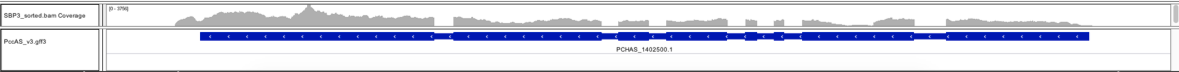
\includegraphics[IGV - PCHAS\_1402500 coverage]{images/answers-coverage.png}
\end{center}


    \hypertarget{q3-do-you-think-this-gene-is-differentially-expressed-and-is-looking-at-the-coverage-plots-alone-a-reliable-way-to-assess-differential-expression}{%
\subsubsection{Q3: Do you think this gene is differentially expressed
and is looking at the coverage plots alone a reliable way to assess
differential
expression?}\label{q3-do-you-think-this-gene-is-differentially-expressed-and-is-looking-at-the-coverage-plots-alone-a-reliable-way-to-assess-differential-expression}}

Possibly. But, you can't tell differential expression by the counts
alone as there may be differences in the sequencing depths of the
samples.

\newpage

    \hypertarget{transcript-quantification-with-kallisto}{%
\subsection{Transcript quantification with
Kallisto}\label{transcript-quantification-with-kallisto}}

\hypertarget{use-kallisto-quant-four-more-times-for-the-mt2-sample-and-the-three-sbp-samples.}{%
\subsubsection{Use kallisto quant four more times, for the MT2 sample
and the three SBP
samples.}\label{use-kallisto-quant-four-more-times-for-the-mt2-sample-and-the-three-sbp-samples.}}

You can run the individual \texttt{kallisto\ quant} commands as you did
for MT1 for each of the remaining samples:

    \begin{tcolorbox}[breakable, size=fbox, boxrule=1pt, pad at break*=1mm,colback=cellbackground, colframe=cellborder]
\prompt{In}{incolor}{ }{\boxspacing}
\begin{Verbatim}[commandchars=\\\{\}]
kallisto quant \PYZhy{}i PccAS\PYZus{}v3\PYZus{}kallisto \PYZhy{}o MT2 \PYZhy{}b \PY{l+m}{100} MT2\PYZus{}1.fastq MT2\PYZus{}2.fastq
kallisto quant \PYZhy{}i PccAS\PYZus{}v3\PYZus{}kallisto \PYZhy{}o SBP1 \PYZhy{}b \PY{l+m}{100} SBP1\PYZus{}1.fastq SBP1\PYZus{}2.fastq
kallisto quant \PYZhy{}i PccAS\PYZus{}v3\PYZus{}kallisto \PYZhy{}o SBP2 \PYZhy{}b \PY{l+m}{100} SBP1\PYZus{}2.fastq SBP2\PYZus{}2.fastq
kallisto quant \PYZhy{}i PccAS\PYZus{}v3\PYZus{}kallisto \PYZhy{}o SBP3 \PYZhy{}b \PY{l+m}{100} SBP1\PYZus{}3.fastq SBP3\PYZus{}2.fastq
\end{Verbatim}
\end{tcolorbox}

    Or, you can write a \texttt{for} loop which will run
\texttt{kallisto\ quant} on all of the samples:

    \begin{tcolorbox}[breakable, size=fbox, boxrule=1pt, pad at break*=1mm,colback=cellbackground, colframe=cellborder]
\prompt{In}{incolor}{ }{\boxspacing}
\begin{Verbatim}[commandchars=\\\{\}]
\PY{k}{for} r1 in *\PYZus{}1.fastq
\PY{k}{do}
  \PY{n+nb}{echo} \PY{n+nv}{\PYZdl{}r1}
  \PY{n+nv}{sample}\PY{o}{=}\PY{l+s+si}{\PYZdl{}\PYZob{}}\PY{n+nv}{r1}\PY{p}{/\PYZus{}1.fastq/}\PY{l+s+si}{\PYZcb{}}
  \PY{n+nb}{echo} \PY{l+s+s2}{\PYZdq{}Quantifying transcripts for sample: \PYZdq{}}\PY{n+nv}{\PYZdl{}sample}
  kallisto quant \PYZhy{}i PccAS\PYZus{}v3\PYZus{}kallisto \PYZhy{}o \PY{n+nv}{\PYZdl{}sample} \PYZhy{}b \PY{l+m}{100} \PY{n+nv}{\PYZdl{}sample}\PY{l+s+s1}{\PYZsq{}\PYZus{}1.fastq\PYZsq{}} \PY{n+nv}{\PYZdl{}sample}\PY{l+s+s1}{\PYZsq{}\PYZus{}2.fastq\PYZsq{}}
\PY{k}{done}
\end{Verbatim}
\end{tcolorbox}

    For more information on how this loop works, have a look at our
\href{../Unix/index.ipynb}{Unix tutorial} and
\href{running-commands-on-multiple-samples.ipynb}{Running commands on
multiple samples}.

    \hypertarget{q1-what-k-mer-length-was-used-to-build-the-kallisto-index}{%
\subsubsection{\texorpdfstring{Q1: What \textit{k}-mer length was used to
build the Kallisto
index?}{Q1: What k-mer length was used to build the Kallisto index?}}\label{q1-what-k-mer-length-was-used-to-build-the-kallisto-index}}

A \textit{k}-mer length of \textbf{31} was used.

Look at the output from \texttt{kallisto\ index}:

\begin{verbatim}
[build] k-mer length: 31
\end{verbatim}

Or, look for the \texttt{-k} or \texttt{-\/-kmer-size} option in the
\texttt{kallisto\ index} usage:

    \begin{tcolorbox}[breakable, size=fbox, boxrule=1pt, pad at break*=1mm,colback=cellbackground, colframe=cellborder]
\prompt{In}{incolor}{ }{\boxspacing}
\begin{Verbatim}[commandchars=\\\{\}]
kallisto index
\end{Verbatim}
\end{tcolorbox}

    \hypertarget{q2-how-many-transcript-sequences-are-there-in-pccas_v3_transcripts.fa}{%
\subsubsection{\texorpdfstring{Q2: How many transcript sequences are
there in
\textit{PccAS\_v3\_transcripts.fa}?}{Q2: How many transcript sequences are there in PccAS\_v3\_transcripts.fa?}}\label{q2-how-many-transcript-sequences-are-there-in-pccas_v3_transcripts.fa}}

There are \textbf{5177} transcript sequences.

Look at the output from \texttt{kallisto\ quant}:

\begin{verbatim}
[index] number of targets: 5,177
\end{verbatim}

Or, look for \textbf{n\_targets} in one of the \textit{run\_info.json}
files:

    \begin{tcolorbox}[breakable, size=fbox, boxrule=1pt, pad at break*=1mm,colback=cellbackground, colframe=cellborder]
\prompt{In}{incolor}{ }{\boxspacing}
\begin{Verbatim}[commandchars=\\\{\}]
cat MT1/run\PYZus{}info.json
\end{Verbatim}
\end{tcolorbox}

    Or, you can run a \texttt{grep} on the transcript FASTA file and count
the number of header lines:

    \begin{tcolorbox}[breakable, size=fbox, boxrule=1pt, pad at break*=1mm,colback=cellbackground, colframe=cellborder]
\prompt{In}{incolor}{ }{\boxspacing}
\begin{Verbatim}[commandchars=\\\{\}]
grep \PYZhy{}c \PY{l+s+s2}{\PYZdq{}\PYZgt{}\PYZdq{}} PccAS\PYZus{}v3\PYZus{}transcripts.fa
\end{Verbatim}
\end{tcolorbox}

    \hypertarget{q3-what-is-the-transcripts-per-million-tpm-value-for-pchas_1402500-in-each-of-the-samples}{%
\subsubsection{Q3: What is the transcripts per million (TPM) value for
PCHAS\_1402500 in each of the
samples?}\label{q3-what-is-the-transcripts-per-million-tpm-value-for-pchas_1402500-in-each-of-the-samples}}

\begin{longtable}[]{@{}cc@{}}
\toprule
Sample & Transcripts Per Million (TPM)\tabularnewline
\midrule
\endhead
MT1 & 2342.23\tabularnewline
MT2 & 1354.42\tabularnewline
SBP1 & 2295.24\tabularnewline
SBP2 & 3274.98\tabularnewline
SBP3 & 2536.17\tabularnewline
\bottomrule
\end{longtable}

You can look at each of the individual abundance files:

    \begin{tcolorbox}[breakable, size=fbox, boxrule=1pt, pad at break*=1mm,colback=cellbackground, colframe=cellborder]
\prompt{In}{incolor}{ }{\boxspacing}
\begin{Verbatim}[commandchars=\\\{\}]
grep \PY{l+s+s2}{\PYZdq{}\PYZca{}PCHAS\PYZus{}1402500\PYZdq{}} MT1/abundance.tsv
grep \PY{l+s+s2}{\PYZdq{}\PYZca{}PCHAS\PYZus{}1402500\PYZdq{}} MT2/abundance.tsv
grep \PY{l+s+s2}{\PYZdq{}\PYZca{}PCHAS\PYZus{}1402500\PYZdq{}} SBP1/abundance.tsv
grep \PY{l+s+s2}{\PYZdq{}\PYZca{}PCHAS\PYZus{}1402500\PYZdq{}} SBP2/abundance.tsv
grep \PY{l+s+s2}{\PYZdq{}\PYZca{}PCHAS\PYZus{}1402500\PYZdq{}} SBP3/abundance.tsv
\end{Verbatim}
\end{tcolorbox}

    Or you can use a recursive \texttt{grep}:

    \begin{tcolorbox}[breakable, size=fbox, boxrule=1pt, pad at break*=1mm,colback=cellbackground, colframe=cellborder]
\prompt{In}{incolor}{ }{\boxspacing}
\begin{Verbatim}[commandchars=\\\{\}]
grep \PYZhy{}r \PY{l+s+s2}{\PYZdq{}\PYZca{}PCHAS\PYZus{}1402500\PYZdq{}} .
\end{Verbatim}
\end{tcolorbox}

    Or you can use a loop:

    \begin{tcolorbox}[breakable, size=fbox, boxrule=1pt, pad at break*=1mm,colback=cellbackground, colframe=cellborder]
\prompt{In}{incolor}{ }{\boxspacing}
\begin{Verbatim}[commandchars=\\\{\}]
\PY{k}{for} r1 in *\PYZus{}1.fastq
\PY{k}{do}
  \PY{n+nv}{sample}\PY{o}{=}\PY{l+s+si}{\PYZdl{}\PYZob{}}\PY{n+nv}{r1}\PY{p}{/\PYZus{}1.fastq/}\PY{l+s+si}{\PYZcb{}}
  \PY{n+nb}{echo} \PY{n+nv}{\PYZdl{}sample}
  grep PCHAS\PYZus{}1402500 \PY{n+nv}{\PYZdl{}sample}\PY{l+s+s1}{\PYZsq{}/abundance.tsv\PYZsq{}}
\PY{k}{done}
\end{Verbatim}
\end{tcolorbox}

    For more information on how this loop works, have a look at our
\href{../Unix/index.ipynb}{Unix tutorial} and
\href{running-commands-on-multiple-samples.ipynb}{Running commands on
multiple samples}.

    \hypertarget{q4-do-you-think-pchas_1402500-is-differentially-expressed}{%
\subsubsection{Q4: Do you think PCHAS\_1402500 is differentially
expressed?}\label{q4-do-you-think-pchas_1402500-is-differentially-expressed}}

Probably not. We would need to run statistical tests to really be sure
though.

\newpage

    \hypertarget{identifying-differentially-expressed-genes-with-sleuth}{%
\subsection{Identifying differentially expressed genes with
Sleuth}\label{identifying-differentially-expressed-genes-with-sleuth}}

    \hypertarget{q1-is-our-gene-from-earlier-pchas_1402500-significantly-differentially-expressed}{%
\subsubsection{Q1: Is our gene from earlier, PCHAS\_1402500,
significantly differentially
expressed?}\label{q1-is-our-gene-from-earlier-pchas_1402500-significantly-differentially-expressed}}

\textbf{No.}

Look at the transcript table.


\begin{center}
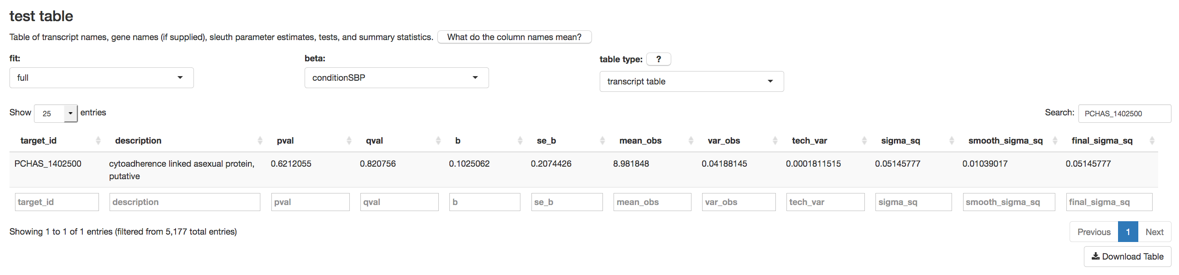
\includegraphics[sleuth - PCHAS\_1402500]{images/sleuth-pchas1402500-table.png}
\end{center}


And the transcript view.


\begin{center}
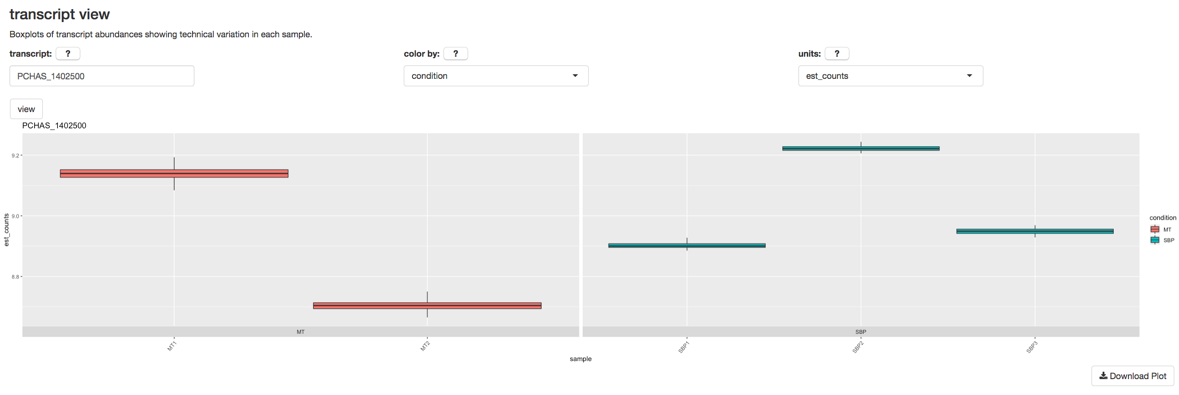
\includegraphics[sleuth - PCHAS\_1402500]{images/sleuth-pchas1402500-view.png}
\end{center}


Although this gene looked like it was differentially expressed from the
plots in IGV, our test did not show it to be so (q-value \textgreater{}
0.05). This might be because some samples tended to have more reads, so
based on raw read counts, genes generally look up-regulated in the SBP
samples.

Alternatively, the reliability of only two biological replicates and the
strength of the difference between the conditions was not sufficient to
be statistically convincing. In the second case, increasing the number
of biological replicates would give us more confidence about whether
there really was a difference.

In this case, it was the lower number of reads mapping to MT samples
that mislead us in the IGV view. Luckily, careful normalisation and
appropriate use of statistics saved the day!

    \begin{tcolorbox}[breakable, size=fbox, boxrule=1pt, pad at break*=1mm,colback=cellbackground, colframe=cellborder]
\prompt{In}{incolor}{ }{\boxspacing}
\begin{Verbatim}[commandchars=\\\{\}]
grep PCHAS\PYZus{}1402500 kallisto.results \PY{p}{|} cut \PYZhy{}f1,4
\end{Verbatim}
\end{tcolorbox}

\newpage

    \hypertarget{interpreting-the-results}{%
\subsection{Interpreting the results}\label{interpreting-the-results}}

\hypertarget{q1-how-many-genes-are-more-highly-expressed-in-the-sbp-samples}{%
\subsubsection{Q1: How many genes are more highly expressed in the SBP
samples?}\label{q1-how-many-genes-are-more-highly-expressed-in-the-sbp-samples}}

\textbf{127}. We can use \texttt{awk} to filter our Kallisto/sleuth
results and \texttt{wc\ -l} to count the number of lines returned.

    \begin{tcolorbox}[breakable, size=fbox, boxrule=1pt, pad at break*=1mm,colback=cellbackground, colframe=cellborder]
\prompt{In}{incolor}{ }{\boxspacing}
\begin{Verbatim}[commandchars=\\\{\}]
awk \PYZhy{}F\PY{l+s+s2}{\PYZdq{}\PYZbs{}t\PYZdq{}} \PY{l+s+s1}{\PYZsq{}\PYZdl{}4 \PYZlt{} 0.01 \PYZam{}\PYZam{} \PYZdl{}5 \PYZgt{} 0\PYZsq{}} kallisto.results \PY{p}{|} wc \PYZhy{}l
\end{Verbatim}
\end{tcolorbox}

    \hypertarget{q2-how-many-genes-are-more-highly-expressed-in-the-mt-samples}{%
\subsubsection{Q2: How many genes are more highly expressed in the MT
samples?}\label{q2-how-many-genes-are-more-highly-expressed-in-the-mt-samples}}

\textbf{169}. We can use \texttt{awk} to filter our Kallisto/sleuth
results and \texttt{wc\ -l} to count the number of lines returned.

    \begin{tcolorbox}[breakable, size=fbox, boxrule=1pt, pad at break*=1mm,colback=cellbackground, colframe=cellborder]
\prompt{In}{incolor}{ }{\boxspacing}
\begin{Verbatim}[commandchars=\\\{\}]
awk \PYZhy{}F\PY{l+s+s2}{\PYZdq{}\PYZbs{}t\PYZdq{}} \PY{l+s+s1}{\PYZsq{}\PYZdl{}4 \PYZlt{} 0.01 \PYZam{}\PYZam{} \PYZdl{}5 \PYZlt{} 0\PYZsq{}} kallisto.results \PY{p}{|} wc \PYZhy{}l
\end{Verbatim}
\end{tcolorbox}

    \hypertarget{q3-do-you-notice-any-particular-genes-that-come-up-in-the-analysis}{%
\subsubsection{Q3: Do you notice any particular genes that come up in
the
analysis?}\label{q3-do-you-notice-any-particular-genes-that-come-up-in-the-analysis}}

Genes from the \textbf{\textit{cir}} family are upregulated in the MT
samples.

To get this we must first find out which genes (or gene descriptions)
are seen most often in the genes which are more highly expressed in our
SBP samples.

    \begin{tcolorbox}[breakable, size=fbox, boxrule=1pt, pad at break*=1mm,colback=cellbackground, colframe=cellborder]
\prompt{In}{incolor}{ }{\boxspacing}
\begin{Verbatim}[commandchars=\\\{\}]
awk \PYZhy{}F\PY{l+s+s2}{\PYZdq{}\PYZbs{}t\PYZdq{}} \PY{l+s+s1}{\PYZsq{}\PYZdl{}4 \PYZlt{} 0.01 \PYZam{}\PYZam{} \PYZdl{}5 \PYZgt{} 0 \PYZob{}print \PYZdl{}2\PYZcb{}\PYZsq{}} kallisto.results \PY{p}{|} sort \PY{p}{|} uniq \PYZhy{}c \PY{p}{|} sort \PYZhy{}nr
\end{Verbatim}
\end{tcolorbox}

    Then, we summarise the genes more highly expressed in our MT samples.

    \begin{tcolorbox}[breakable, size=fbox, boxrule=1pt, pad at break*=1mm,colback=cellbackground, colframe=cellborder]
\prompt{In}{incolor}{ }{\boxspacing}
\begin{Verbatim}[commandchars=\\\{\}]
awk \PYZhy{}F\PY{l+s+s2}{\PYZdq{}\PYZbs{}t\PYZdq{}} \PY{l+s+s1}{\PYZsq{}\PYZdl{}4 \PYZlt{} 0.01 \PYZam{}\PYZam{} \PYZdl{}5 \PYZlt{} 0 \PYZob{}print \PYZdl{}2\PYZcb{}\PYZsq{}} kallisto.results \PY{p}{|} sort \PY{p}{|} uniq \PYZhy{}c \PY{p}{|} sort \PYZhy{}nr
\end{Verbatim}
\end{tcolorbox}

    Perhaps the CIR proteins are interesting. There are only 2 CIR proteins
upregulated in the SBP samples and 25 CIR in the MT samples.

The \textbf{\textit{cir}} family is a large, malaria-specific gene family
which had previously been proposed to be involved in immune evasion
(Lawton et al., 2012). Here, however, we see many of these genes
upregulated in a form of the parasite which seems to cause the immune
system to better control the parasite. This suggests that these genes
interact with the immune system in a subtler way, preventing the immune
system from damaging the host.

\newpage

    \hypertarget{normalisation}{%
\subsection{Normalisation}\label{normalisation}}

\hypertarget{how-we-got-the-information-to-help-the-questions}{%
\subsubsection{How we got the information to help the
questions}\label{how-we-got-the-information-to-help-the-questions}}

To answer the questions you needed the following for each sample:

\begin{itemize}
\tightlist
\item
  Number of reads assigned to PCHAS\_1402500
\item
  Length of exons in PCHAS\_1402500 (bp)
\item
  Total number of reads mapping
\item
  Total RPK
\end{itemize}

First, take a quick look at the first five lines of the
\texttt{abundance.tsv} for MT1.

    \begin{tcolorbox}[breakable, size=fbox, boxrule=1pt, pad at break*=1mm,colback=cellbackground, colframe=cellborder]
\prompt{In}{incolor}{ }{\boxspacing}
\begin{Verbatim}[commandchars=\\\{\}]
head \PYZhy{}5 MT1/abundance.tsv
\end{Verbatim}
\end{tcolorbox}

    There are five columns which give us information about the transcript
abundances for our MT1 sample.

\begin{longtable}[]{@{}ll@{}}
\toprule
\begin{minipage}[b]{0.47\columnwidth}\raggedright
Column\strut
\end{minipage} & \begin{minipage}[b]{0.47\columnwidth}\raggedright
Description\strut
\end{minipage}\tabularnewline
\midrule
\endhead
\begin{minipage}[t]{0.47\columnwidth}\raggedright
target\_id\strut
\end{minipage} & \begin{minipage}[t]{0.47\columnwidth}\raggedright
Unique transcript identifier\strut
\end{minipage}\tabularnewline
\begin{minipage}[t]{0.47\columnwidth}\raggedright
length\strut
\end{minipage} & \begin{minipage}[t]{0.47\columnwidth}\raggedright
Number of bases found in exons.\strut
\end{minipage}\tabularnewline
\begin{minipage}[t]{0.47\columnwidth}\raggedright
eff\_length\strut
\end{minipage} & \begin{minipage}[t]{0.47\columnwidth}\raggedright
\textit{Effective length}. Uses fragment length distribution to determine
the effective number of positions that can be sampled on each
transcript.\strut
\end{minipage}\tabularnewline
\begin{minipage}[t]{0.47\columnwidth}\raggedright
est\_counts\strut
\end{minipage} & \begin{minipage}[t]{0.47\columnwidth}\raggedright
\textit{Estimated counts}. This may not always be an integer as reads
which map to multiple transcripts are fractionally assigned to each of
the corresponding transcripts.\strut
\end{minipage}\tabularnewline
\begin{minipage}[t]{0.47\columnwidth}\raggedright
tpm\strut
\end{minipage} & \begin{minipage}[t]{0.47\columnwidth}\raggedright
\textit{Transcripts per million}. Normalised value accounting for length
and sequence depth bias.\strut
\end{minipage}\tabularnewline
\bottomrule
\end{longtable}

First, look for your gene of interest, \textbf{PCHAS\_1402500}. Run this
as a loop to \texttt{grep} the information for all five samples.

    \begin{tcolorbox}[breakable, size=fbox, boxrule=1pt, pad at break*=1mm,colback=cellbackground, colframe=cellborder]
\prompt{In}{incolor}{ }{\boxspacing}
\begin{Verbatim}[commandchars=\\\{\}]
\PY{k}{for} r1 in *\PYZus{}1.fastq
\PY{k}{do}
  \PY{n+nv}{sample}\PY{o}{=}\PY{l+s+si}{\PYZdl{}\PYZob{}}\PY{n+nv}{r1}\PY{p}{/\PYZus{}1.fastq/}\PY{l+s+si}{\PYZcb{}}
  \PY{n+nb}{echo} \PY{n+nv}{\PYZdl{}sample}
  grep PCHAS\PYZus{}1402500 \PY{n+nv}{\PYZdl{}sample}\PY{l+s+s1}{\PYZsq{}/abundance.tsv\PYZsq{}}
\PY{k}{done}
\end{Verbatim}
\end{tcolorbox}

    Now you have the length (eff\_length) and counts (est\_counts) for
PCHAS\_1402500 for each of your samples. Next, you need to get the total
number of reads mapped to each of your samples. You can use a loop to do
this.

In the loop below \texttt{samtools\ flagstat} gives you the number of
mapped paired reads (reads with itself and mate mapped) and those where
one read mapped but its mate didn't (singletons). If then uses
\texttt{grep} to get the relevant lines and \texttt{awk} to add the
mapped paired and singleton read totals together.

    \begin{tcolorbox}[breakable, size=fbox, boxrule=1pt, pad at break*=1mm,colback=cellbackground, colframe=cellborder]
\prompt{In}{incolor}{ }{\boxspacing}
\begin{Verbatim}[commandchars=\\\{\}]
\PY{k}{for} r1 in *\PYZus{}1.fastq
\PY{k}{do}
  \PY{n+nv}{sample}\PY{o}{=}\PY{l+s+si}{\PYZdl{}\PYZob{}}\PY{n+nv}{r1}\PY{p}{/\PYZus{}1.fastq/}\PY{l+s+si}{\PYZcb{}}

  \PY{n+nv}{total}\PY{o}{=}\PY{l+s+sb}{`} samtools flagstat \PY{n+nv}{\PYZdl{}sample}\PY{l+s+s1}{\PYZsq{}\PYZus{}sorted.bam\PYZsq{}} \PY{p}{|} \PY{l+s+se}{\PYZbs{}}
          grep \PY{l+s+s1}{\PYZsq{}singletons\PYZbs{}|with itself and mate mapped\PYZsq{}} \PY{p}{|} \PY{l+s+se}{\PYZbs{}}
          awk \PY{l+s+s1}{\PYZsq{}BEGIN\PYZob{} count=0\PYZcb{} \PYZbs{}}
\PY{l+s+s1}{               \PYZob{}count+=\PYZdl{}1\PYZcb{} \PYZbs{}}
\PY{l+s+s1}{               END\PYZob{}print count\PYZcb{}\PYZsq{}}\PY{l+s+sb}{`}

  \PY{n+nb}{echo} \PYZhy{}e \PY{l+s+s2}{\PYZdq{}}\PY{n+nv}{\PYZdl{}sample}\PY{l+s+s2}{\PYZbs{}t}\PY{n+nv}{\PYZdl{}total}\PY{l+s+s2}{\PYZdq{}}
\PY{k}{done}
\end{Verbatim}
\end{tcolorbox}

    Finally, to calculate the TPM values, you need the total RPK for each of
your samples. Again we use a loop. Notice the use of
\texttt{NR\textgreater{}2} in the \texttt{awk} command which tells it to
skip the two header lines at the start of the file. You will also notice
that we divide the eff\_length by 1,000 so that it's in kilobases.

    \begin{tcolorbox}[breakable, size=fbox, boxrule=1pt, pad at break*=1mm,colback=cellbackground, colframe=cellborder]
\prompt{In}{incolor}{ }{\boxspacing}
\begin{Verbatim}[commandchars=\\\{\}]
\PY{k}{for} r1 in *\PYZus{}1.fastq
\PY{k}{do}
  \PY{n+nv}{sample}\PY{o}{=}\PY{l+s+si}{\PYZdl{}\PYZob{}}\PY{n+nv}{r1}\PY{p}{/\PYZus{}1.fastq/}\PY{l+s+si}{\PYZcb{}}

  awk \PYZhy{}F\PY{l+s+s2}{\PYZdq{}\PYZbs{}t\PYZdq{}} \PYZhy{}v \PY{n+nv}{sample}\PY{o}{=}\PY{l+s+s2}{\PYZdq{}}\PY{n+nv}{\PYZdl{}sample}\PY{l+s+s2}{\PYZdq{}} \PY{l+s+se}{\PYZbs{}}
      \PY{l+s+s1}{\PYZsq{}BEGIN\PYZob{}total\PYZus{}rpk=0;\PYZcb{} \PYZbs{}}
\PY{l+s+s1}{       NR\PYZgt{}2 \PYZbs{}}
\PY{l+s+s1}{       \PYZob{} \PYZbs{}}
\PY{l+s+s1}{         rpk=\PYZdl{}4/(\PYZdl{}3/1000); \PYZbs{}}
\PY{l+s+s1}{         total\PYZus{}rpk+=rpk \PYZbs{}}
\PY{l+s+s1}{       \PYZcb{} \PYZbs{}}
\PY{l+s+s1}{       END\PYZob{}print sample\PYZdq{}\PYZbs{}t\PYZdq{}total\PYZus{}rpk\PYZcb{}\PYZsq{}} \PY{n+nv}{\PYZdl{}sample}\PY{l+s+s1}{\PYZsq{}/abundance.tsv\PYZsq{}}
\PY{k}{done}
\end{Verbatim}
\end{tcolorbox}

    \hypertarget{q1-using-the-abundance.tsv-files-generated-by-kallisto-and-the-information-above-calculate-the-rpkm-for-pchas_1402500-in-each-of-our-five-samples.}{%
\subsubsection{\texorpdfstring{Q1: Using the \texttt{abundance.tsv}
files generated by Kallisto and the information above, calculate the
RPKM for PCHAS\_1402500 in each of our five
samples.}{Q1: Using the abundance.tsv files generated by Kallisto and the information above, calculate the RPKM for PCHAS\_1402500 in each of our five samples.}}\label{q1-using-the-abundance.tsv-files-generated-by-kallisto-and-the-information-above-calculate-the-rpkm-for-pchas_1402500-in-each-of-our-five-samples.}}

\begin{longtable}[]{@{}ccccc@{}}
\toprule
\begin{minipage}[b]{0.17\columnwidth}\centering
Sample\strut
\end{minipage} & \begin{minipage}[b]{0.17\columnwidth}\centering
Per million scaling factor\strut
\end{minipage} & \begin{minipage}[b]{0.17\columnwidth}\centering
Reads per million (RPM)\strut
\end{minipage} & \begin{minipage}[b]{0.17\columnwidth}\centering
Per kilobase scaling factor\strut
\end{minipage} & \begin{minipage}[b]{0.17\columnwidth}\centering
RPKM\strut
\end{minipage}\tabularnewline
\midrule
\endhead
\begin{minipage}[t]{0.17\columnwidth}\centering
MT1\strut
\end{minipage} & \begin{minipage}[t]{0.17\columnwidth}\centering
2.353750\strut
\end{minipage} & \begin{minipage}[t]{0.17\columnwidth}\centering
1079.528\strut
\end{minipage} & \begin{minipage}[t]{0.17\columnwidth}\centering
3.697\strut
\end{minipage} & \begin{minipage}[t]{0.17\columnwidth}\centering
\textbf{292}\strut
\end{minipage}\tabularnewline
\begin{minipage}[t]{0.17\columnwidth}\centering
MT2\strut
\end{minipage} & \begin{minipage}[t]{0.17\columnwidth}\centering
2.292271\strut
\end{minipage} & \begin{minipage}[t]{0.17\columnwidth}\centering
1479.581\strut
\end{minipage} & \begin{minipage}[t]{0.17\columnwidth}\centering
3.709\strut
\end{minipage} & \begin{minipage}[t]{0.17\columnwidth}\centering
\textbf{398}\strut
\end{minipage}\tabularnewline
\begin{minipage}[t]{0.17\columnwidth}\centering
SBP1\strut
\end{minipage} & \begin{minipage}[t]{0.17\columnwidth}\centering
2.329235\strut
\end{minipage} & \begin{minipage}[t]{0.17\columnwidth}\centering
6270.170\strut
\end{minipage} & \begin{minipage}[t]{0.17\columnwidth}\centering
3.699\strut
\end{minipage} & \begin{minipage}[t]{0.17\columnwidth}\centering
\textbf{1695}\strut
\end{minipage}\tabularnewline
\begin{minipage}[t]{0.17\columnwidth}\centering
SBP2\strut
\end{minipage} & \begin{minipage}[t]{0.17\columnwidth}\centering
2.187718\strut
\end{minipage} & \begin{minipage}[t]{0.17\columnwidth}\centering
7908.652\strut
\end{minipage} & \begin{minipage}[t]{0.17\columnwidth}\centering
3.696\strut
\end{minipage} & \begin{minipage}[t]{0.17\columnwidth}\centering
\textbf{2140}\strut
\end{minipage}\tabularnewline
\begin{minipage}[t]{0.17\columnwidth}\centering
SBP3\strut
\end{minipage} & \begin{minipage}[t]{0.17\columnwidth}\centering
2.163979\strut
\end{minipage} & \begin{minipage}[t]{0.17\columnwidth}\centering
6767.949\strut
\end{minipage} & \begin{minipage}[t]{0.17\columnwidth}\centering
3.699\strut
\end{minipage} & \begin{minipage}[t]{0.17\columnwidth}\centering
\textbf{1830}\strut
\end{minipage}\tabularnewline
\bottomrule
\end{longtable}

\hypertarget{q2-using-the-abundance.tsv-files-generated-by-kallisto-and-the-information-above-calculate-the-tpm-for-pchas_1402500-in-each-of-our-five-samples.}{%
\subsubsection{\texorpdfstring{Q2: Using the \texttt{abundance.tsv}
files generated by Kallisto and the information above, calculate the TPM
for PCHAS\_1402500 in each of our five
samples.}{Q2: Using the abundance.tsv files generated by Kallisto and the information above, calculate the TPM for PCHAS\_1402500 in each of our five samples.}}\label{q2-using-the-abundance.tsv-files-generated-by-kallisto-and-the-information-above-calculate-the-tpm-for-pchas_1402500-in-each-of-our-five-samples.}}

\begin{longtable}[]{@{}cccc@{}}
\toprule
Sample & Per kilobase scaling factor & Reads per kilobase (RPK) &
TPM\tabularnewline
\midrule
\endhead
MT1 & 3.697 & 687.30 & \textbf{2342}\tabularnewline
MT2 & 3.709 & 914.50 & \textbf{1354}\tabularnewline
SBP1 & 3.699 & 3947.87 & \textbf{2295}\tabularnewline
SBP2 & 3.696 & 4681.81 & \textbf{3275}\tabularnewline
SBP3 & 3.699 & 3959.78 & \textbf{2536}\tabularnewline
\bottomrule
\end{longtable}

\hypertarget{q3-do-these-match-the-tpm-values-from-kallisto}{%
\subsubsection{Q3: Do these match the TPM values from
Kallisto?}\label{q3-do-these-match-the-tpm-values-from-kallisto}}

\textbf{Yes.}

Well, almost. They may be a couple out because we rounded up to make the
calculations easier.

    \hypertarget{q4-do-you-think-pchas_1402500-is-differentially-expressed-between-the-mt-and-sbp-samples}{%
\subsubsection{Q4: Do you think PCHAS\_1402500 is differentially
expressed between the MT and SBP
samples?}\label{q4-do-you-think-pchas_1402500-is-differentially-expressed-between-the-mt-and-sbp-samples}}

\textbf{Probably not.}

If we were to look at only the counts and RPKM values then it appears
there is an 8 fold difference between the MT and SBP samples. However,
when we look at the TPM values, they are much closer and so differential
expression is less likely.


    % Add a bibliography block to the postdoc



\end{document}
